\documentclass[12pt]{article}

%Required packages
\usepackage[utf8]{inputenc}
\usepackage{apacite}
\usepackage{caption} 
\usepackage{setspace}
\usepackage{amsmath}
\usepackage{graphicx}
\usepackage[textwidth=160mm, textheight=210mm, hmarginratio=1:1]{geometry}


%Prerequisite statements
\captionsetup[table]{skip=4pt} %Line indent after table title
\captionsetup{labelfont={bf}} %Bold label font for tables
\onehalfspacing %Document line spacing
\pagestyle{myheadings} %Heading style
\graphicspath{ {./figures/} } %Defining image path

\begin{document}

%Title page 
\begin{titlepage}
\begin{center}
\LARGE{\textbf{The Realtime Assessment of Mental Workload by Means of Multiple Bio-Signals}}\\
\vspace*{2\baselineskip}
\Large{\textbf{Master thesis Report}}\\
Methodology and Statistics for the Behavioral, Biomedical and Social Sciences\\
\vspace*{1\baselineskip}
Utrecht University\\
\vspace*{4\baselineskip}
{Bart-Jan Boverhof, 6000142}\\
\vspace*{1\baselineskip}
{\textbf{Thesis Supervisor}}\\
Prof.dr.ir. B.P. Veldkamp\\
\vspace*{1\baselineskip}
{\textbf{Date}}\\
October 14, 2020\\
\vspace*{1\baselineskip}
\end{center}
\end{titlepage}

\section{Introduction} \label{Introduction}
The topic of mental workload (MWL) has received widespread attention across a variety of different fields, amongst others the field of ergonomics \cite{young2015state}, human factors \cite{pretorius2007development} and neurosciences \cite{shuggi2017mental}.
A simple definition of MWL is the demand placed upon humans whilst carrying out a certain task. As pointed out by de Waard (1996), such a definition is too shallow, for it defines workload solely in external sense. It is of importance to acknowledge that MWL is person-specific, for the amount of experienced MWL ushered by a given task may differ across people \cite{de1996measurement}. When referring to MWL throughout this research, person-specific MWL is meant specifically.

A commonly employed measure of workload is the NASA-Task Load Index (or TLX) questionnaire, operationalizing workload in clusters of six different dimensions \cite{hart2006nasa}. Such measurements are usually conducted post experiment, which could introduce some bias. An example of such a bias is the observer bias, prescribing that actors participating in an experiment tend to over-exaggerate the treatment effect when having to report it themselves post-experiment \cite{mahtani2018catalogue}.

An alternative method for assessing MWL is by measuring bio-signals during the experiment, and use these to classify the degree of perceived MWL. Examples of such bio-signals (hereafter modalities) include techniques such as electroencephalogram, eye tracking, galvanic skin response, functional near-infrared spectroscopy, etc. The advantage of an approach like this is that complementary information streams, each stemming from a different modality can be interpreted simultaneously \cite{ramachandram2017deep}. This yields an objective and rich multifaceted classification of a mental construct, such as MWL. Additionally, a separate model for each respondent individually can be fitted, catering towards the individual perception of MWL. This approach comes however at the cost of an increase in complexity. This complexity resides in the construction of a complex framework that inputs the data from the utilized modalities, and outputs a single classification outcome. 

The current research directly builds upon previous research conducted by Dolmans and colleagues, who proposed a framework for multi-modal deep-learning classification of MWL \cite{dolmans2020perceived}. The current research will explore the feasibility of a similar framework, but by utilizing different modalities and data. Additionally a realtime component will be introduced. This implies that classification can done in realtime, that is whilst the experiment takes place, opening the possibility for the researcher to alter the state of the experiment in realtime. Such an approach could enable a wide range of possibilities: consider for example a flight simulation with the objective of educating pilots. The possibility for such a simulation to be altered dynamically could substantially enhance the learning-experience, namely by catering the state of the simulation towards the the individual, for example based on their perceived workload. 

In order to build both frameworks, three of the (arguably) most widely utilized modalities will be included. These modalities include the techniques of electroencephalogram (EEG), galvanic skin response (GSR) and photoplethysmography (PPG). It is important to stress that the objective of the current research is not to gain insight into the most optimal model design for each of the previously delineated modalities. It is rather to construct a framework with which realtime classification can be managed, and to which modalities of choice can easily be added. Consequently, one of two design principles on which the architecture of the framework reclines is the concept of modularity. Modularity refers the extent to which different modalities can freely be added and/or removed, without the necessity to re-architect and rebuild the framework. The second adhered design principle is the principle generalizability, prescribing that the framework should not solely be utilizable in the context of MWL, but also for the measurement of other mental constructs.

Considering the relative complexity of a multi-modular deep neural network, an important point of attention is model optimization. In order for realtime classification to be a feasible, an optimized and swift neural network is required. The problem in realtime classification with deep learning is often not the quality of classification, but rather the speed of classification. The focus of the current research is therefore to architect and optimize a multi-modular deep neural network, which is capable of realtime classification, whilst still ensuring ample accuracy in classification. Several networks will be investigated upon in order to asses this. Ultimately, this line of research pursues the ability to conduct a dynamic experiment for multiple people simultaneously, the state of which can be altered in real-time. 

\newpage
\section{Methods}

\subsection{Related Work} \label{Relatedwork}
The current section will provide an overview of previous research on the model design for each seperate modality. Additionally,  the most feasible architecture for a multi-modular framework will be explored. In particular, attention is placed upon the data fusion, the real-time component and several model optimization techniques.

\subsubsection{First modality: Electroencephalogram (EEG)}
The first utilized modality is EEG, which detects electrical activity in the brain using electrodes. EEG is a widely utilized method for classifying MWL during experiments. With their review of the complete literature on EEG classification with deep learning, \citeA{craik2019deep} found a total of 16 \% of all available papers to deal with MWL, lending credence to the ability of EEG for classifying MWL. Additionally, the usage of deep learning for a range of different EEG application was mapped. Summarizing, it was reported that studies mostly found deep belief networks and convolutional neural networks (ConvNets) to perform best when classifying workload, and advice one of these approaches consequently \cite{craik2019deep}.

Research by \citeA{schirrmeister2017deep} contrasted the performance of several ConvNets against the widely acknowledged baseline method for EEG data, being FBCSP. The investigated networks included deep, shallow, deep-shallow hybrid and residual ConvNets. Both the deep and shallow ConvNets were found to reach at least similar, and in some regard better classification results, as compared with the FBCSP baseline. Altogether, a deep ConvNet with four convolutional-max-pooling blocks was found to perform best, displaying an accuracy of 92.4 \% \cite{schirrmeister2017deep}. The appropriate design choices were found to be of importance in order to be able to reach this accuracy, including the employment of techniques such as batch normalization, dropout and the usage of the ELU activation function.

A different approach is proposed by \citeA{tabar2016novel}, combining a ConvNet with a Stacked auto-encoder network (SAE). Within this network, the input layer feeds into a convolutional layer with the objective of learning the filters and network parameters. The output of this convolutional layer subsequently feeds into SAE part of the network, constituting an input layer, 6 hidden layers and an output layer. A classification accuracy of 90 \% was acquired with this model \cite{tabar2016novel} . 

\subsubsection{Second modality: Galvanic Skin Response (GSR)}
The second utilized modality is GSR, measuring sweat gland on the hands and hereby inferring arousal. GSR readings have been found to significantly increase as a consequence of an increase in task cognitive load, hence constituting to be an objective predictor \cite{shi2007galvanic}. 

Sun and colleagues explored the most optimal deep-learning model for classifying six different emotional states by means of GSR data. Several models were investigated, amongst others the support vector machine, the ConvNet, the long-short-term-memory (LSTM) model and a hybrid model combining the ConvNet and LSTM approaches. The hybrid model was found to perform best, exhibiting an accuracy of 74\%. Additionally, data augmentation was found to be able to substantially increase classification results \cite{sun2019hybrid}. 

A variant on the CovNet LSTM model was employed by \citeA{dolmans2020perceived}, who aimed to classify MWL by means of amongst other modalities GSR (equally so as the current research). The performance of this model was contrasted with a network consisting solely of fully connected dense layers. Conform with findings by Sun and colleagues, the hybrid model was found to perform best \cite{dolmans2020perceived}, displaying an accuracy of 82 \%. The model architecture as utilized by Dolmans and colleagues deployed 2 convolutional layers, after each of which batch normalization was performed. Subsequently, max pooling was performed, after which the network feeds into two LSTM layers, followed by a dense layer.

\subsubsection{Third modality: Photoplethysmography (PPG)}
The third modality constitutes PPG, which is a technique utilized to measure heart rate. PPG is, not undeservedly, a widely deployed technique within the field of MWL classification. Zhang and colleagues investigated several approaches for measuring MWL, amongst three others the technique of PPG. Out of these four approaches, PPG was found to display both the highest sensitivity and reliability for measuring MWL, lending credence to the feasibility of PPG as a method for classifying MWL \cite{zhang2018evaluating}. 

Work by Biswas and colleagues investigated a deep learning approach to PPG data, with the objective to perform both bio-metric identification and heart rate information. Exceptional results were attained with a neural network, attaining an average accuracy of 96 \% \cite{biswas2019cornet}. This performance was managed with a hybrid model, incorporating two convolutional, followed with two LSTM layers. After each of two convolutional layers, batch normalisation and max pooling was applied. 

The previously delineated model as proposed by Biswas and colleagues was adopted by Dolmans and colleagues, and subsequently applied towards the MWL case. This neural network was contrasted with a network of two fully connected dense layers. Batch normalisation and max pooling was performed in both contrasted networks. Surprisingly, the more sophisticated network constituting of the convolutional and LSTM layers was found to perform worse in the context of MLW classification, as compared with the simpler model, solely build from two dense layers \cite{dolmans2020perceived}.   

\subsubsection{Fusion strategy}  
When architecting a multi-model framework, it is of importance to realize that the information stemming from the different modalities are required to be combined (i.e. fused) in order to ultimately result in a single classification. Fusion can be done at different time-points within the framework. Several fusion strategies as proposed by Ramachandram and colleagues will be considered \cite{ramachandram2017deep}.

Early (or data-level) fusion focuses on how to optimally combine data sources, before being fed into the classification model. Techniques that realize this include for example principle component analysis or factor analysis. Early fusing is usually challenging, especially in a multimodal scenario such as the current. This resides in the fact that data stemming from different modalities differ substantially in terms of dimensionality and sampling rate. Another disadvantage of early fusing, is that usually the oversimplified assumption of conditional independence is made. This assumption is unrealistic, for data stemming from different modalities are expected to be correlated in practice \cite{ramachandram2017deep}. 

Late (or decision level) fusion on the other hand, refers to the process of aggregating the decisions from multiple models, each individually trained on all modalities. In case the data sources stemming from the various modalities are either correlated or measured within a deviant dimensionality, late fusion is a much more feasible approach \cite{ramachandram2017deep}.

Lastly, intermediate fusion is the most widely employed fusion strategy for multi-modal deep-learning problems. Modalities are fused by simply adding a higher order layer, to which the individual deep-learning models separately defined for each modality feed into. This need not be a single layer, but could also be multiple layers, as long as each modality ultimately feeds into the highest order output layer. The depth of the fusion (i.e. the amount of fusion layers) can be chosen conform the specific situation, posing intermediate fusion to be the most flexible, and therefore the most widely used fusion method \cite{ramachandram2017deep}.

Indeed, when consulting the literature, intermediate fusion strategies are the most prevailing for multimodal deep neural networks. When taking such an approach, one is required to design the architecture of these fusion layers.  \citeA{rastgoo2019automatic} utilize a multimodal ConvNet approach, and fuse the modalities by concatenation followed by two LTSM layers, 2 dense layers and a softmax layer. A simpler approach is utilized by	\citeA{han2020classification}, who utilized an intermediate fusion approach solely consisting of several fully connected dense layers, ended with a soft-max layer. Lastly, \citeA{dolmans2020perceived} used a much more deeper intermediate fusion approach, consisting of two dense layers, two convolutional layers followed by another two dense layers.  

\subsubsection{Model optimization}
The technique of batch normalization was proposed by  \citeA{ioffe2015batch},  and is often applied in deep learning with the objective of enhancing the stability of a network. This is endeavored by including a batch normalization layer after each convolutional layer, re-centering and re-scaling the input feeding into this layer. If incorporating a batch normalization layer, it is recommended to do so before feeding into the activation function \cite{ioffe2015batch}. An increase in accuracy for EEG classification was attained by \citeA{dolmans2020perceived},  \citeA{schirrmeister2017deep} by specifying a batch normalization layer after each convolutional layer. Equally so, the best performing model for PPG data as proposed by \citeA{biswas2019cornet} included a batch normalization layer after each convolutional layer.  

Pooling layers are often used in ConvNets, following a convolutional layer with the attempt to decrease the dimensionality. The objective of such layers are to merge similar features into one (for a more extensive elaboration see: \cite{lecun2015deep}). Considering the EEG ConvNets, both \citeA{schirrmeister2017deep} and \citeA{tabar2016novel} specified a max-pooling layer after each convolutional layer. The model proposed for GSR data by \citeA{sun2019hybrid} incorporate a max-pooling layer after each, but one of the convolutional layers. Lastly, the model as proposed for PPG data by \cite{biswas2019cornet}  specified a max pooling layer after each convolutional layer. 

Hyper-parameter optimization (HPO) is a technique that can be used to optimize hyper-parameter including learning rate, dropout probability and momentum. The Optuna toolbox provides a method for creating a parameter search space, from which values for the hyper-parameters can be sampled \cite{akiba2019optuna}. 

\subsection{Data}
The current section will provide an overview of the utilized data. Special attention is placed on the experimental setup, the description of the participants and the data collection / synchronization process. 

\subsubsection{Experimental setup}
The experimental setting for data collection is the spaceship videogame Empty Epsilon, in which the respondent is required to carry out tasks on a virtual spaceship \cite{daid2016empty}. This experiment is instituted by the Brain Computer Interfaces (BCI) testbed lab, hosted by the University of Twente (UT) and carried out in cooperation with Thales group Hengelo. The experiment constituted three different segments, during each of which respondents had to carry out different tasks, all aiming to measure workload. Each segment consists of six small sessions of roughly 5-10 minutes. These sessions varied in difficulty, including two easy, two intermediate and two hard sessions per segment. A schematic overview of the experimental structure is depicted as table \ref{table:expsetup}. After each of the 18 segments, respondents filled in the TLX questionnaire consisting of 6 questions each, resulting in 18 filled in questionnaires. Each questionnaire inquired upon the degree to which the respondent experienced workload during the previous session. These ratings will be used as labels in later training. Within each segment, the order in which the sessions (varying in difficulty) were presented have been randomized. The order in which the segments were administrated were not random. Between every three sessions, respondents were requested to take a short 2 minute break.
\bigskip
\bgroup
\def\arraystretch{1.6}%  
\begin{table}[h]
\centering
\caption{Experimental setup: Number of sessions per segment and difficulty setting}
\label{table:expsetup}
\begin{tabular}{llll}
                               & Easy                   & Intermediate           & Hard                   \\ \cline{2-4} 
\multicolumn{1}{l|}{Segment 1} & \multicolumn{1}{l|}{2} & \multicolumn{1}{l|}{2} & \multicolumn{1}{l|}{2} \\ \cline{2-4} 
\multicolumn{1}{l|}{Segment 2} & \multicolumn{1}{l|}{2} & \multicolumn{1}{l|}{2} & \multicolumn{1}{l|}{2} \\ \cline{2-4} 
\multicolumn{1}{l|}{Segment 3} & \multicolumn{1}{l|}{2} & \multicolumn{1}{l|}{2} & \multicolumn{1}{l|}{2} \\ \cline{2-4} 
\end{tabular}
\end{table}
\egroup
\bigskip 

The first segment emulated a scenario in which hostile spaceships approach the respondents spaceship. The respondent is required to  quickly react, and defuse hostile spaceships in order to survive. The increment in difficulty caused the process of defusing hostile spaceships to be more challenging and hereby to take longer,  aiming to increase workload consequently. The second segment emulated a scenario in which the respondent had to navigate their spaceship trough space, gathering as many way-points as possible. Obstacles around which the respondent had to carefully navigate were introduced in the intermediate difficult scenario, and hostile spaceships the respondent had to decimate were introduced in the hard scenario. Both increase difficulty, and hereby aim to increase workload consequently. The third and final segment emulated a machine room, in which respondents had to control the power based on random requests generated by the video-game. Variables that could overheat the spaceship  were introduced as a consequence of an increase in difficulty, demanding the respondent multi-task, hereby aiming to increase workload. 

\subsubsection{Participants}
In total, twenty-five respondents are participating in the study. Currently, the data is still in the process of being collected, for which no additional descriptive statistics can be presented in the prevailing section. The respondents are students, recruited from the University of Twente. Recruitment has been conducted with Sona, which is a cloud-based participant management system. Requirements were that respondents didn't have constraints that might interfere with the utilized sensors, such as for example a pacemaker. This is assessed by means of a short demographic questionnaire prior to the experiment. Additionally, the respondents are made aware of ethical consent prior to the experiment, with the objective to ensure completely voluntary participation. Respondents were able to draw back from the experiment at any time. 

\subsubsection{Devices and Synchronization}
The Shimmer3 GSR+ sensor is used for both PPG and GSR measurements. The device is worn on the wrist, and communicates the signals wirelessly. An ear-clip is utilized for measuring the PPG, and converting this to estimate heart rate. Skin conductivity (GSR) is monitored between two electrodes attached to two fingers \cite{shimmer}. Both PPG and GSR are measured on a sample rate of 256 Hz, i.e. 256 measured data points per second. EEG measurement is conducted with the shimmer 2, equally so on a sampling rate of 256 Hz.

Data streams stemming from the different modalities are measured on different frequencies, and consequently need to be properly synchronized. This is accomplished by means of an application called Lab-Streaming Layer (LSL), to which different data streams are streamed during the experiment. LSL properly synchronizes these data streams such that they refer to the same points in time, and records all data into a single file per participant \cite{kothe2018lab}.

\subsection{Framework Architecture}

\subsubsection{Universal Framework Architecture}
The architecture for the proposed framework is constructed by combining insights from the literature whilst keeping in mind the previously delineated design principles (i.e. the principles of modularity and generalizability). No variations based on the general framework architecture will be made, for deviating from the architecture as verified in the literature is likely to be detrimental towards classification accuracy.

The utilized network for the EEG modality is a ConvNet as proposed by \citeA{schirrmeister2017deep}. The network is designed to include four convolutional layers, each follow by a max pooling layer of stride 3. The Exponential Linear Unit (ELU) function is utilized as activation function, defined as: 

\begin{equation}
f(x)= 
\begin{Bmatrix}
x & x \geq0 \\ 
\alpha (e^x -1) & x<0
\end{Bmatrix}
\bigskip
\end{equation}

The utilized network for the GSR modality is a LSTM ConvNet hybrid model, inspired by the work of \citeA{sun2019hybrid} and  \citeA{dolmans2020perceived}. The network is designed to include two convolutional blocks, each consisting of a convolutional layer, followed by a batch normalization layer and closed with a max-pooling layer of stride 4. Following these blocks are two LTSM layers. The Rectified Linear Unit (ReLU) function is utilized as activation function, defined as: 

\begin{equation} 
\label{eqn:relu}
f(x)=max(0,x)
\bigskip
\end{equation}

Lastly, the PPG modality is analyzed by means of the model as proposed by \citeA{biswas2019cornet}. The nework starts with two convolutional blocks, each consisting of a convolutional layer, batch normalization layer and closed with a max pooling layer of stride 4. Following these blocks are two LTSM layers, equal to the GSR model. The utilized activation function is the ReLU, depicted as equation \ref{eqn:relu}.

The network for each of the modalities are finally closed with one fully connected dense layer before feeding into the head network, such that all inputs are flattened in a lower dimensional space. All outputs from these dense layers are concatenated. The head network consists of Four dense layers, alternated with some batch normalization and max-pooling layers with the objective of stabilization. A visual representation of the utilized model is depicted as figure \ref{fig:architecture}.

\begin{figure}
\caption{Framework Architecture}
\bigskip
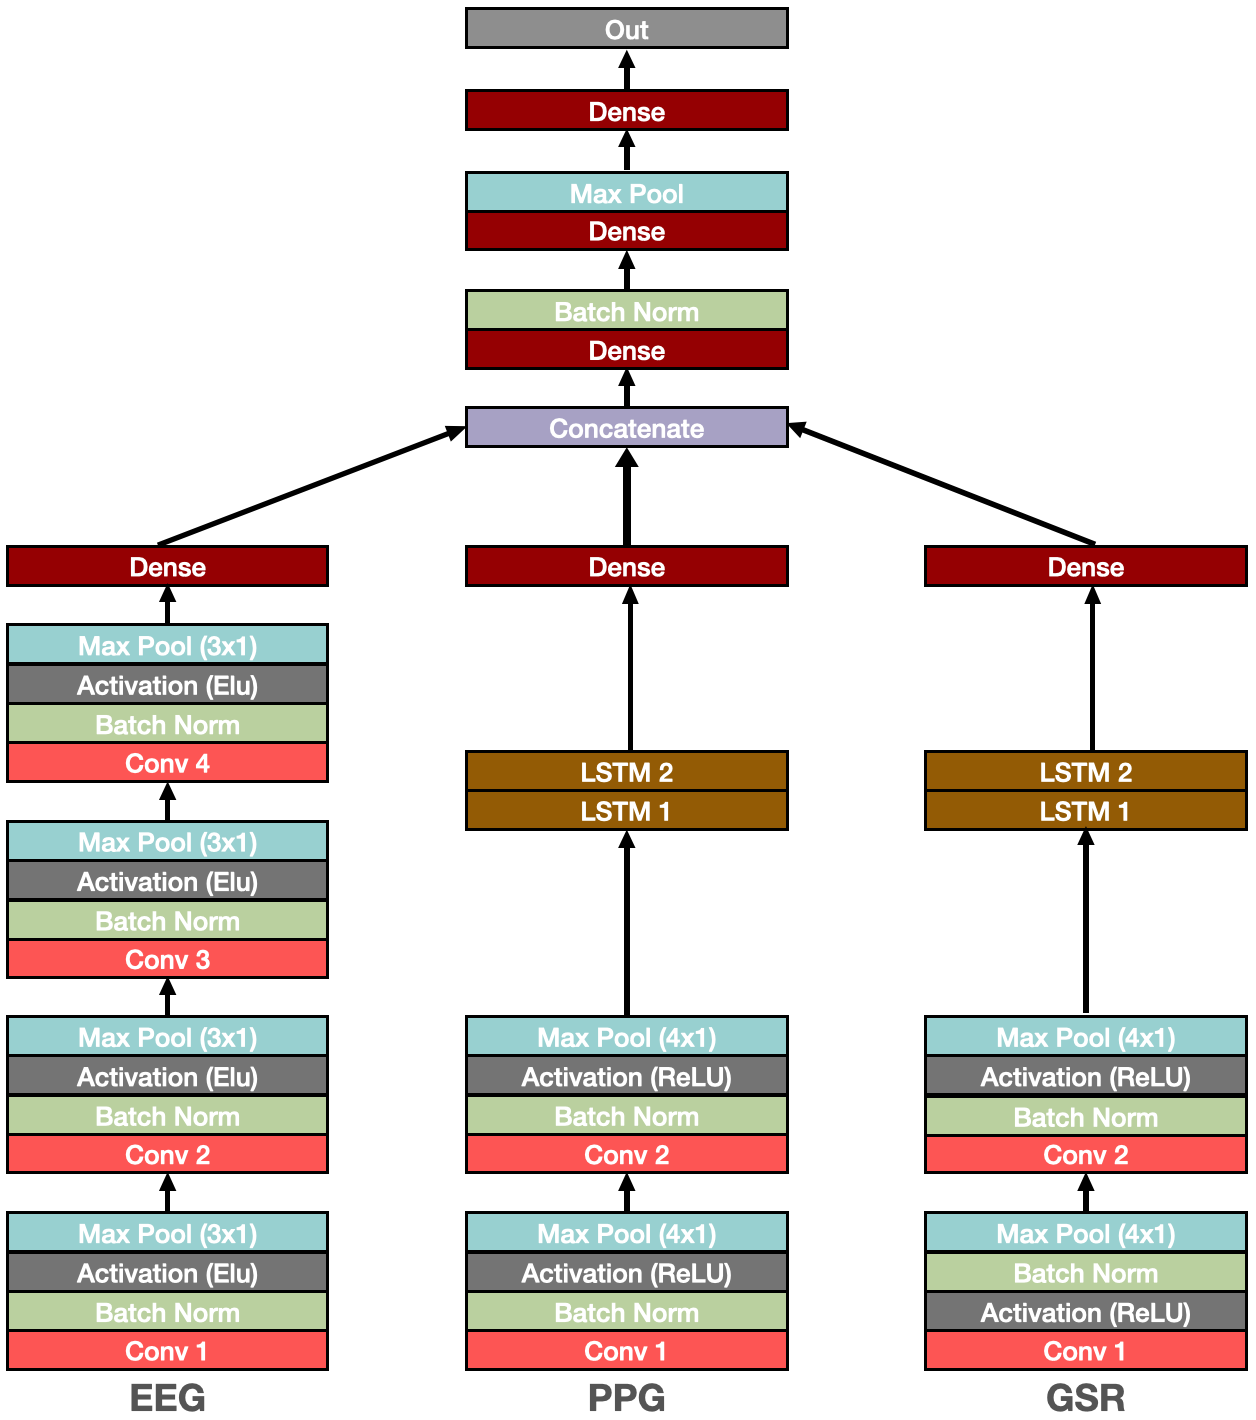
\includegraphics[scale=0.725]{model_architecture}
\label{fig:architecture}
\end{figure}


\subsubsection{Model Variations}
Multi-modular classification in realtime by means of deep-learning requires an optimized network, as was elaborated upon in the introduction. Speed is a potential bottleneck for realtime classification with deep learning, especially given the fact the proposed framework architecture is multi-modular, and consequently very complex. Different model variations will be investigated upon as a consequence of this. The aim is to propose a model that is fast enough for realtime classification, whilst ensuring the maximum amount of accuracy. Variations on two different parameters of the previously delineated model will therefore be considered, resulting in four different models. 

The first variation reflects the sample rates for each of the included modalities. As was elaborated on before, the data collection for each modality was on a sampling rate of 256Hz. Naturally, an increase in speed can be attained by feeding less data into the model, i.e. decreasing the sampling rate. Two out of the four models will consequently model based on a sampling rate of 256Hz, whilst the other two models will model based on sampling rate of 128Hz. 

The second variation reflects the amount of utilized filters for convolutional layers, and the amount of neurons for all utilized layers. A decrease in the amount of filters / neurons equals a decrease in network size, and consequently an increase in speed. Two out of the four models will be the full sized network, whilst the other two models will be halved in size. An overview of all four models and their size is provided in table \ref{table:modelvariations}.
\bigskip

\bgroup
\def\arraystretch{1.6}%  
\begin{table}[h]
\centering
\caption{Model variations	}
\label{table:modelvariations}
\begin{tabular}{lllll}
\hline
                   & EEG        & GSR        & PPG        & Head       \\ \hline
Model 1: 128Hz \&  & Conv1: 25  & Conv1: 128 & Conv1: 128 & Dense: 712 \\
Model 2: 256Hz     & Conv2: 50  & Conv2: 128 & Conv2: 128 & Dense: 356 \\
                   & Conv3: 100 & LSTM1: 256 & LSTM1: 256 & Dense: 178 \\
                   & Conv4: 200 & LSTM1: 256 & LSTM2: 256 &            \\
                   \vspace{3ex}
                   & Dense: 200 & Dense: 256 & Dense: 256 &            \\
Model 3: 128 Hz \& & Conv1: 13  & Conv1: 64  & Conv1: 64  & Dense: 356 \\
Model 4: 256Hz     & Conv2: 25  & Conv2: 64  & Conv2: 64  & Dense: 178 \\
                   & Conv3: 50  & LSTM1: 128 & LSTM1: 128 & Dense: 89  \\
                   & Conv4: 100 & LSTM1: 128 & LSTM2: 128 &            \\
                   & Dense: 100 & Dense: 128 & Dense: 128 &            \\ \hline
\end{tabular}
\vspace{2ex}

{\raggedright \textit{Note: for convolutional layers the provided number reflects the amount of filters, whereas for all other layers it refers to the amount of nodes.} \par}
\end{table}
\egroup

\subsection{Model Evaluation}
The performance of the real-time framework will be assessed by contrasting it with a regular, non-real-time framework. Specifically, the quality of performance for each modality individually will be compared across both frameworks. This validation will be endeavored by means of six widely used performance measures, all constructed from the confusion matrix, depicted as table  \ref{table:confusion}  
\bigskip
\bgroup
\def\arraystretch{1.6}%  
\begin{table}[h]
\centering
\caption{Confusion matrix}
\label{table:confusion}
\begin{tabular}{lll}
                                        & True Positive          & True Negative          \\ \cline{2-3} 
\multicolumn{1}{l|}{Predicted Positive} & \multicolumn{1}{l|}{a} & \multicolumn{1}{l|}{b} \\ \cline{2-3} 
\multicolumn{1}{l|}{Predicted Negative} & \multicolumn{1}{l|}{c} & \multicolumn{1}{l|}{d} \\ \cline{2-3} 
\end{tabular}
\end{table}
\egroup

The measures accuracy, sensitivity, specificity, PPV, NPV and F1 will be utilized in order to asses model performance. The framework that performs best across these measures is considered to be the superior performing framework. Table \ref{table:metrics} depicts the constitution of these performance measures by partly referring to confusion matrix depicted as table \ref{table:confusion}. 
\bigskip
\bgroup
\def\arraystretch{1.8}%  
\begin{table}[h]
\centering
\caption{Performance Metrics}
\label{table:metrics}
\begin{tabular}{ll}
\hline
Accuracy:                       & \(\frac{\!\!\!\!\!\!\!\!\!\!\!\!\!\!a+d}{a+b+c+d}\) \\
Sensitivity:                    & \(\frac{a}{a+c}\)                                   \\
Specificity:                    & \(\frac{d}{b+d}\)                                   \\
Positive Predicted Value (PPV): & \(\frac{a}{a+b}\)                                   \\
Negative Predicted Value:       & \(\frac{d}{c+d}\)                                   \\
F1-measure:                     & \(\frac{2*Sensitivity*PPV}{Sensitivity+PPV}\)       \\ \hline
\end{tabular}
\end{table}
\egroup

\newpage

\bibliographystyle{apacite}
\bibliography{References}

\end{document}
